\documentclass[11pt]{article}
\usepackage[a4paper,margin=1in]{geometry}
\usepackage{amsmath,amssymb,amsthm}
\usepackage{tikz}
\usepackage{booktabs}
\usepackage[hidelinks]{hyperref}
\hypersetup{pdftitle={Which orders maximise the span of a chain?},pdfauthor={Vamshi Jandhyala}}
\setlength{\parskip}{0.4em}
\setlength{\parindent}{0pt}

\newtheorem{theorem}{Theorem}
\newtheorem{lemma}{Lemma}[section]
\newtheorem{proposition}[lemma]{Proposition}
\newtheorem{corollary}[lemma]{Corollary}
\newtheorem{conjecture}{Conjecture}
\theoremstyle{remark}
\newtheorem*{remark}{Remark}
\newcommand{\cC}{\mathcal C}
\DeclareMathOperator{\rev}{rev}

\title{Which orders maximise the span of a chain?}
\author{Vamshi Jandhyala}
\date{}

\begin{document}
\maketitle
\vspace{-2em}

\begin{abstract}
A planar chain is built from $n$ segments of given distinct lengths, joined so that each turns anticlockwise by one of $n-1$ given distinct angles. Lengths and angles may be used in any order. Which orders make the distance from start to end as large as possible? We prove that, when the angles total less than $\pi$, every optimal chain has strictly unimodal lengths with the two shortest at the ends, turns that fall to a minimum and then rise, and its longest segment at the smallest turn. This confirms observations of Chaunier and leads to an algorithm with $O(n^2\log n\,2^n)$ arithmetic operations. For the counting question of Moura and Garcia, where the angles total at most $\pi/2$, we show that exactly three relative orders occur for four segments, and that for every $n$ at least $b_n$ orders occur, where $b_n=1,3,6,14,31,70,157,\dots$ is OEIS A006356. We conjecture equality. The structure theorem and the case of four segments are formally verified in Lean.
\end{abstract}

\section{The question}

Take three sticks of lengths $1$, $2$ and $3$, and two angles, $\alpha\approx16.3^\circ$ and $\beta\approx36.9^\circ$. Lay one stick down, turn anticlockwise by one of the angles, lay the next stick from its end, turn by the other angle, and lay the last stick. How should you order the sticks and the angles to end up as far from the start as possible?

\emph{Before reading on, guess.} A natural guess is to lead with the longest stick and the smallest angle, so that the long pieces point roughly the same way.

\begin{figure}[ht]
\centering
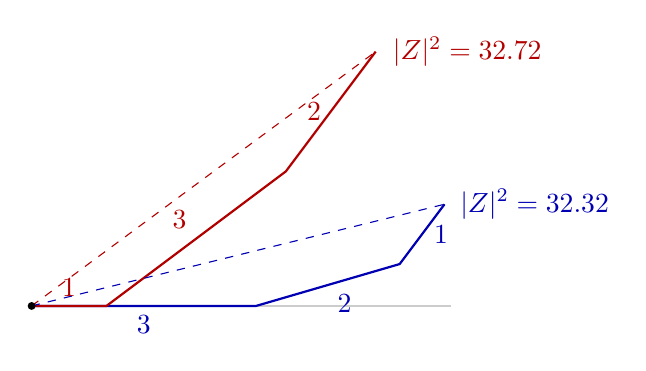
\begin{tikzpicture}[scale=0.95]
\draw[gray!40] (0,0) -- (5.6,0);
\draw[thick,blue!70!black] (0,0) -- (3,0) -- (4.92,0.56) -- (5.52,1.36);
\draw[thick,red!70!black] (0,0) -- (1,0) -- (3.4,1.8) -- (4.6,3.4);
\draw[dashed,blue!70!black] (0,0) -- (5.52,1.36);
\draw[dashed,red!70!black] (0,0) -- (4.6,3.4);
\fill (0,0) circle (1.5pt);
\node[below,blue!70!black] at (1.5,0) {$3$};
\node[below right,blue!70!black] at (3.96,0.28) {$2$};
\node[right,blue!70!black] at (5.25,0.96) {$1$};
\node[above,red!70!black] at (0.5,0) {$1$};
\node[above left,red!70!black] at (2.2,0.9) {$3$};
\node[left,red!70!black] at (4.0,2.6) {$2$};
\node[blue!70!black,right] at (5.6,1.36) {$|Z|^2=32.32$};
\node[red!70!black,right] at (4.7,3.4) {$|Z|^2=32.72$};
\end{tikzpicture}
\caption{Lengths $1,2,3$ and turns $\alpha=\arcsin\frac{7}{25}$, $\beta=\arcsin\frac45-\arcsin\frac7{25}$. Blue: longest first, then the smaller turn. Red: shortest first, then the larger turn, then the longest segment. The red chain ends farther away; it is the best of all six orders.}
\label{fig:three}
\end{figure}

Figure~\ref{fig:three} shows that the guess loses. The best chain starts with the \emph{shortest} stick, turns by the \emph{larger} angle, and puts the longest stick in the middle. The picture shows why. Each stick contributes according to how closely it lines up with the final direction of travel, and that direction lies in the middle of the fan of directions, so the middle is where the longest stick belongs.

The question for general $n$ goes back to two 2012 posts by Tom\'as~\cite{tomas-mse,tomas-mo}. MvG answered the fixed-turn-order version with a sweep over projection directions~\cite{mvg}. In 2023 Moura posed the counting form on MathOverflow, attributing the problem to Ronaldo Garcia~\cite{moura}: the lengths and angles are arbitrary distinct positive numbers, the angles total at most $\pi/2$, and the question is how many relative orders, $a_n$, can be optimal, and which ones. From random searches Moura found $a_3=1$, $a_4\ge3$, $a_5\ge6$, $a_6\ge14$ and $a_7\ge29$, and Claude Chaunier observed that the optimal length orders all seemed unimodal with the two shortest lengths at the ends, and the turn orders unimodal too.

This paper proves those observations, with the turns falling and then rising, under the weaker assumption that the angles total less than $\pi$; settles $a_4=3$; and gives an explicit recursive family of optimal orders that shows $a_n\ge b_n$ for every $n$, where $b_n$ is OEIS A006356. Two members of the family for $n=7$ are missing from Moura's list, so $a_7\ge31$.

\subsection*{Notation}

Fix $n\ge2$ and data
\begin{equation}\label{eq:data}
0<L_0<\cdots<L_{n-1},\qquad 0<A_0<\cdots<A_{n-2},\qquad T=A_0+\cdots+A_{n-2}<\pi .
\end{equation}
An \emph{arrangement} is a pair of permutations, $p$ of $\{0,\dots,n-1\}$ and $q$ of $\{0,\dots,n-2\}$. Segment $i$ has length $l_i=L_{p_i}$; the turn after it is $a_i=A_{q_i}$. Segment $i$ points in direction $\theta_i=a_0+\cdots+a_{i-1}$ (so $\theta_0=0$ and $\theta_{n-1}=T$), and the chain's displacement and span are
\begin{equation}\label{eq:span}
Z=\sum_{i=0}^{n-1} l_i\,e^{i\theta_i},\qquad |Z|.
\end{equation}
In words: $Z$ is the sum of the segments as vectors, and $|Z|$ is the distance from start to end. An arrangement is \emph{optimal} if no other arrangement of the same data has a larger span. Reversing both lists gives the mirror image of the chain, $e^{iT}\overline{Z}$, with the same span; we usually normalise so that the shortest length comes first. We write arrangements as rank lists, so $(021,10)$ is the red chain of Figure~\ref{fig:three}.

\subsection*{Results}

\begin{theorem}[Structure]\label{thm:structure}
Assume~\eqref{eq:data} with $n\ge3$. In every optimal arrangement:
\begin{enumerate}
\item the lengths increase strictly to their maximum and then decrease strictly;
\item the two shortest lengths are at the two ends;
\item the turns decrease strictly to their minimum and then increase strictly (either part may be empty);
\item the longest segment is one of the two segments at the smallest turn.
\end{enumerate}
With the shortest length first, the first turn descends and, if $n\ge4$, the last turn ascends.
\end{theorem}

\begin{theorem}[Algorithm]\label{thm:algorithm}
The maximum span can be found with $O(n^2\log n\,2^n)$ arithmetic operations and comparisons, and $O(n^2)$ storage.
\end{theorem}

\begin{theorem}[Counting]\label{thm:counting}
Let $a_n$ be the number of normalised arrangements that are optimal for some data with $T\le\pi/2$. Then $a_1=a_2=a_3=1$, $a_4=3$, and $a_n\ge b_n$ for every $n$, where $b_3=1$, $b_4=3$, $b_5=6$ and
\[
b_n=2b_{n-1}+b_{n-2}-b_{n-3}\qquad(n\ge6),
\]
so $b_n=1,3,6,14,31,70,157,353,\dots$ for $n=3,4,5,\dots$ (OEIS A006356~\cite{oeis}). For $n\ge4$, $a_n\le 2\binom{2n-5}{n-3}-2$.
\end{theorem}

\begin{conjecture}\label{conj}
$a_n=b_n$ for every $n$: the optimal arrangements are exactly the recursive family $\cC_n$ of Section~\ref{sec:family}.
\end{conjecture}

The growth rate of $b_n$ is $1/(2\cos(3\pi/7))\approx2.247$. The upper bound grows like $4^n$, so the gap is large; Section~\ref{sec:open} explains why the natural local arguments cannot close it.

\section{The supporting direction}\label{sec:support}

Everything rests on one observation. Let $\varphi=\arg Z$ be the direction of travel of an optimal chain. Among all arrangements, the optimal one must also go farthest \emph{in the direction} $\varphi$; otherwise some other chain would project farther onto $\varphi$ and so be longer. Projection onto a fixed direction is linear in the segments, so local changes become easy to compare.

All directions $\theta_i$ lie in $[0,T]$, an arc shorter than a half-turn, so $Z\neq0$ and $0<\varphi<T$ (the imaginary parts of $Z$ and of $e^{-iT}Z$ are a positive and a negative sum).

\begin{lemma}[Support]\label{lem:support}
If $Z$ is optimal and $\varphi=\arg Z$, every arrangement $Z'$ of the same data satisfies $\operatorname{Re}(e^{-i\varphi}Z')\le|Z|$, with equality only if $Z'=Z$.
\end{lemma}

\begin{proof}
$\operatorname{Re}(e^{-i\varphi}Z')\le|Z'|\le|Z|$. Equality throughout forces $e^{-i\varphi}Z'$ to be the positive real number $|Z|$, so $Z'=Z$.
\end{proof}

The projection of segment $i$ onto $\varphi$ is $l_i\cos(\theta_i-\varphi)$. Two moves change only a few of these terms.

\begin{lemma}[Length exchange]\label{lem:length}
At an optimum, $(l_i-l_j)\bigl(\cos(\theta_i-\varphi)-\cos(\theta_j-\varphi)\bigr)>0$ for $i\ne j$. Equivalently, longer segments point strictly closer to $\varphi$: $l_i>l_j$ if and only if $|\theta_i-\varphi|<|\theta_j-\varphi|$.
\end{lemma}

\begin{proof}
Swapping $l_i$ and $l_j$ changes $Z$ by $(l_j-l_i)(e^{i\theta_i}-e^{i\theta_j})$ and the projection by $(l_j-l_i)(\cos(\theta_i-\varphi)-\cos(\theta_j-\varphi))$, which Lemma~\ref{lem:support} makes non-positive. Equality would leave $Z$ unchanged, impossible as $l_i\neq l_j$ and $0\le\theta_i,\theta_j<\pi$ are distinct. Since $|\theta-\varphi|<\pi$, a larger cosine means a smaller angular distance.
\end{proof}

\begin{lemma}[Turn exchange]\label{lem:turn}
At an optimum, $(a_k-a_{k+1})(\theta_k+\theta_{k+2}-2\varphi)<0$ for $0\le k\le n-3$.
\end{lemma}

\begin{proof}
Swapping $a_k$ and $a_{k+1}$ moves only segment $k+1$, from direction $\theta_k+a_k$ to $\theta_k+a_{k+1}$. By Lemma~\ref{lem:support} and the identity $\cos x-\cos y=-2\sin\frac{x+y}2\sin\frac{x-y}2$,
\[
0\ \ge\ \cos(\theta_k+a_{k+1}-\varphi)-\cos(\theta_k+a_k-\varphi)
=-2\sin\Bigl(\frac{\theta_k+\theta_{k+2}}2-\varphi\Bigr)\sin\frac{a_{k+1}-a_k}2 ,
\]
and equality is excluded as before. Both sines have arguments in $(-\pi,\pi)$, so the two arguments have the same sign.
\end{proof}

Read Lemma~\ref{lem:turn} as a test on the midpoint $m_k=(\theta_k+\theta_{k+2})/2$ of the two directions around the pair of turns: a descent $a_k>a_{k+1}$ is allowed only when $m_k<\varphi$, an ascent only when $m_k>\varphi$. Figure~\ref{fig:fan} shows both lemmas at once.

\begin{figure}[ht]
\centering
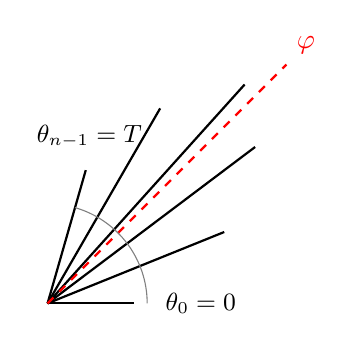
\begin{tikzpicture}[scale=1.1]
\foreach \t/\l/\c in {0/1.0/0, 22/2.2/1, 37/3.0/2, 48/3.4/3, 60/2.6/4, 74/1.6/5} {
  \draw[thick] (0,0) -- (\t:\l);
}
\draw[red,dashed,thick] (0,0) -- (45:3.9) node[above right] {$\varphi$};
\draw[gray] (0:1.15) arc (0:74:1.15);
\node at (0:1.25) [right] {\small $\theta_0=0$};
\node at (74:1.75) [above] {\small $\theta_{n-1}=T$};
\end{tikzpicture}
\caption{A schematic chain satisfying every conclusion of Theorem~\ref{thm:structure}, its segments drawn from a common origin in their directions $\theta_i$. The direction of travel $\varphi$ lies inside the fan, past its middle; lengths grow towards $\varphi$ and shrink away from it (Lemma~\ref{lem:length}), so they rise and then fall along the chain.}
\label{fig:fan}
\end{figure}

\section{Proof of the structure theorem}\label{sec:structure}

The strategy is to read off each part from the two exchange lemmas, using one more move, at the ends of the chain, to locate $\varphi$ precisely.

\emph{Lengths.} As $i$ increases, $\theta_i$ increases, so $|\theta_i-\varphi|$ decreases and then increases. By Lemma~\ref{lem:length} the lengths increase strictly and then decrease strictly, and the shortest length is at an end, the one farther from $\varphi$. Normalise so that it is first. Then $\theta_0=0$ is farther from $\varphi$ than $\theta_{n-1}=T$, that is
\begin{equation}\label{eq:half}
\varphi>T/2 .
\end{equation}

\emph{The far end.} Moving the first segment, with the turn after it, to the end of the chain gives a legal arrangement. Write $Z=l_0+e^{ia_0}W$, where $W$ is the displacement of the rest of the chain measured from its own first direction; the moved chain has displacement $W+l_0e^{iT}$. Put $\gamma=(T+a_0)/2$, $\delta=(T-a_0)/2$ and $V=e^{-i\delta}W$, so that $e^{ia_0}W=e^{i\gamma}V$ and $e^{-iT}W=e^{-i\gamma}V$. Expanding the squared norms,
\[
|Z|^2-|W+l_0e^{iT}|^2=2l_0\bigl(\operatorname{Re}(e^{i\gamma}V)-\operatorname{Re}(e^{-i\gamma}V)\bigr)=-4l_0\sin\gamma\,\operatorname{Im}V .
\]
Optimality makes this non-negative, and $0<\gamma<\pi$, so $\operatorname{Im}V\le0$. Then
\[
\operatorname{Im}\bigl(e^{-i\gamma}Z\bigr)=-l_0\sin\gamma+\operatorname{Im}V<0 ,
\]
which says that $Z$ lies clockwise of the direction $\gamma$:
\begin{equation}\label{eq:endpoint}
\varphi<\frac{T+a_0}{2} .
\end{equation}
Every direction other than $\theta_0$ lies in $[a_0,T]$, and by~\eqref{eq:endpoint} the end $T$ is strictly farther from $\varphi$ than $a_0$ is. So segment $n-1$ points farthest from $\varphi$ among the segments after the first, and by Lemma~\ref{lem:length} it is the second shortest. This proves part~2.

\emph{Turns.} The midpoints $m_k$ increase with $k$. By Lemma~\ref{lem:turn}, a descent needs $m_k<\varphi$ and an ascent needs $m_k>\varphi$, so every descent comes before every ascent. This is part~3.

\emph{The longest segment.} Let $a_z$ be the smallest turn. If $z>0$, the descent before it gives $\theta_{z-1}+\theta_{z+1}<2\varphi$, so $\theta_z$ is closer to $\varphi$ than every earlier direction. If $z<n-2$, the ascent after it gives $\theta_z+\theta_{z+2}>2\varphi$, so $\theta_{z+1}$ is closer than every later direction. The direction closest to $\varphi$ is therefore $\theta_z$ or $\theta_{z+1}$, and Lemma~\ref{lem:length} puts the longest segment there. This is part~4.

\emph{First and last turns.} An ascent at $k=0$ would need $\theta_2>2\varphi>T$ by~\eqref{eq:half}, impossible. For $n\ge4$, a descent at $k=n-3$ would need $\theta_{n-3}+T<2\varphi<T+a_0$ by~\eqref{eq:endpoint}, impossible since $\theta_{n-3}\ge\theta_1=a_0$. This completes the proof of Theorem~\ref{thm:structure}.

\begin{remark}
The bound $T<\pi$ cannot simply be dropped. With lengths $1,2,3$ and turns $2\arctan3$ and $2\arctan4$ (total more than $\pi$), the squared spans of the six orders are $\frac{26}{85},\frac{68}{85},\frac{234}{85},\frac{290}{85},\frac{900}{85},\frac{914}{85}$, and the best, $(102,10)$, puts the shortest segment in the middle.
\end{remark}

\section{An exponential algorithm}\label{sec:algorithm}

For a fixed turn order, MvG's method~\cite{mvg} finds the best length order: for a trial direction $\psi$, the projection $\sum l_i\cos(\theta_i-\psi)$ is maximised by giving longer lengths to directions closer to $\psi$, and that assignment changes only when $\psi$ passes a midpoint $(\theta_i+\theta_j)/2$, where two segments swap rank. Sweeping $\psi$ across $[0,T]$ visits at most $\binom n2$ events; maintaining $Z$ through each swap costs $O(1)$ by the update $Z\leftarrow Z+(l_j-l_i)(e^{i\theta_i}-e^{i\theta_j})$. The optimum's own direction $\varphi$ is not an event (Lemma~\ref{lem:length}), so the sweep meets the optimal length order on an open interval of $\psi$ and evaluates it.

Theorem~\ref{thm:structure} cuts the outer loop over turn orders from $(n-1)!$ to the valley orders. Normalising instead so that the largest turn is first, which a valley order allows since its largest turn is at an end, leaves $2^{n-3}$ turn orders, each needing $O(n^2\log n)$ operations to sort its events. This proves Theorem~\ref{thm:algorithm}. With integer lengths and rational half-angle tangents $\tan(A_j/2)=t_j/d$, every rotation $e^{iA_j}=(d^2-t_j^2+2idt_j)/(d^2+t_j^2)$ is rational, so the events and the spans can be ordered exactly in integer arithmetic; the programs accompanying this paper do this.

\section{Counting optimal orders}\label{sec:counting}

\emph{An upper bound.} With the shortest length first, Theorem~\ref{thm:structure} leaves length orders $(0,S^{\uparrow},n-1,S^{c\downarrow},1)$ with $S\subseteq\{2,\dots,n-2\}$, and valley turn orders whose first turn descends and last turn ascends, with the turn minimum next to the length peak. If the peak is in position $k$ there are $\binom{n-3}{k-1}$ length orders and $\binom{n-2}{k-1}+\binom{n-2}{k}$ turn orders; summing by Vandermonde's identity and removing the two monotone turn orders gives at most $M_n=2\binom{2n-5}{n-3}-2$ candidates for $n\ge4$. These are necessary conditions only.

\emph{Three segments.} The structure theorem leaves only $(021,10)$, the red chain of Figure~\ref{fig:three}, so $a_3=1$.

\begin{proposition}\label{prop:four}
$a_4=3$. The optimal orders for four segments are $(0231,201)$, $(0321,201)$ and $(0231,102)$.
\end{proposition}

\begin{proof}
The structure theorem leaves the length orders $0231$ and $0321$ and the turn orders $201$ and $102$. The pair $(0321,102)$ is impossible: its two longest segments are at directions $\theta_1=A_1$ and $\theta_2=A_1+A_0$ with the longer first, so Lemma~\ref{lem:length} gives $2\varphi<\theta_1+\theta_2=2A_1+A_0$, while~\eqref{eq:half} gives $2\varphi>A_0+A_1+A_2$; together $A_2<A_1$, a contradiction. Exact witnesses for the other three are in Table~\ref{tab:four}.
\end{proof}

\begin{table}[ht]
\centering
\begin{tabular}{ccccc}
\toprule
$p$ & $q$ & lengths $L$ & tangents $t$ & $d$\\
\midrule
0231 & 201 & $1,2,3,4$ & $1,2,3$ & 10\\
0321 & 201 & $2,3,4,5$ & $1,2,4$ & 10\\
0231 & 102 & $8,9,10,32$ & $2,3,4$ & 20\\
\bottomrule
\end{tabular}
\caption{Witnesses for the three orders with four segments; turns are $A_j=2\arctan(t_j/d)$, all totals below $1.2<\pi/2$. Each order is the unique optimum among all $72$ reversal classes, by margins $\frac{18132}{143117}$, $\frac{1408}{38077}$ and $\frac{148404}{537017}$ in squared span.}
\label{tab:four}
\end{table}

For $n=5,\dots,8$ the same kind of exact witness shows that $6$, $14$, $31$ and $70$ distinct orders are each the unique optimum for some data with $T<\pi/2$. Each witness is checked against every structural candidate in exact integer arithmetic, which by Theorem~\ref{thm:structure} covers all arrangements; for $n\le6$ it is also checked against every arrangement without using the theorem. Moura's list for $n=7$ has $29$ orders~\cite{moura}. The two missing ones are
\[
(0246531,432015)\quad\text{and}\quad(0246531,542013),
\]
with witnesses $L=(27,30,36,346,374,377,1000)$, $t=(94,95,112,113,114,135)$ and $L=(1,23,24,25,26,27,100)$, $t=(100,101,105,106,110,111)$, both with $d=1000$. Each is the unique optimum among all $7!\,6!/2=1{,}814{,}400$ reversal classes, with squared-span margins above $144$ and above $1.39$. So $a_7\ge31$.

\section{A recursive family}\label{sec:family}

The witnesses suggest that every optimal order is built from a smaller one by adding short segments at the ends. Write $P+c$ for adding $c$ to every entry of a list and $\rev P$ for reversal. Let $\cC_1=\{(0;\varnothing)\}$, $\cC_2=\{(01;0)\}$, $\cC_3=\{(021;10)\}$, and for $n\ge4$ let $\cC_n$ consist of:
\begin{enumerate}
\item[(A)] for each $2\le k\le n-1$ and each $(P,Q)\in\cC_{n-k+1}$, the pair
\[
p=(0,\ \rev P+(k-1),\ k-2,k-3,\dots,1),\qquad q=(n-2,\ \rev Q,\ n-k,n-k+1,\dots,n-3);
\]
\item[(B)] for each $(P,Q)\in\cC_{n-2}$, the pair $p=(0,\ P+2,\ 1)$, $q=(n-3,\ Q,\ n-2)$.
\end{enumerate}
In words, (A) puts one new shortest segment and the largest turn in front of the reversed parent, and the remaining $k-2$ new segments behind it in decreasing order, with increasing turns; (B) puts one new segment at each end, with the two largest turns, the smaller in front. For example $\cC_4$ consists of $(0231,201)$ and $(0321,201)$ from (A) and $(0231,102)$ from (B), the three orders of Proposition~\ref{prop:four}.

\begin{proposition}\label{prop:count}
$|\cC_n|=b_n$.
\end{proposition}

\begin{proof}
The two operations produce different first turns, $n-2$ and $n-3$. Every length order in $\cC_m$, $m\ge2$, starts with $0$ and ends with $1$, so the output of (A) determines $k=p_1$ and then $(P,Q)$; (B) is also injective. Hence $|\cC_n|=\sum_{m=2}^{n-1}|\cC_m|+|\cC_{n-2}|$ for $n\ge4$, which gives $1,3,6$ for $n=3,4,5$, and subtracting consecutive identities gives the recurrence of Theorem~\ref{thm:counting}.
\end{proof}

The lower bound in Theorem~\ref{thm:counting} follows from the next theorem.

\begin{theorem}[Realisation]\label{thm:realise}
For every $n$, every $(p,q)\in\cC_n$ and every $0<\tau\le\pi/2$ there are distinct positive lengths and turns, with total turn below $\tau$, for which $(p,q)$ is the unique optimum up to reversal.
\end{theorem}

The idea is to start from data realising the parent and add the new segments with tiny lengths $\varepsilon s_j$. At $\varepsilon=0$ the new segments contribute nothing, and the optimum must contain the parent as a contiguous block using the smallest turns (Lemma~\ref{lem:zero}). To first order in $\varepsilon$ the squared span is $R^2+2\varepsilon RF$, where $R$ is the parent's span and $F$ is the total projection of the new segments onto the parent's direction, so the comparison reduces to maximising the linear quantity $F$; the turns are chosen so that this forces exactly the shape of (A) or (B).

\begin{lemma}[Zero lengths]\label{lem:zero}
Suppose $m\ge2$ lengths are positive and the rest are zero, with distinct positive turns totalling less than $\pi/2$. Then every optimum places the positive segments in one contiguous block using the $m-1$ smallest turns, arranged optimally for those lengths and turns.
\end{lemma}

\begin{proof}
Remove the zero-length segments. Between consecutive positive segments sits a nonempty group of turns. Replacing each group by a single one of its turns, and then the chosen turns by the $m-1$ smallest in the same rank order, decreases every angular separation between positive segments, strictly unless the block was already contiguous with the smallest turns. Every separation is below $\pi/2$, and in $|Z|^2=\sum l_i^2+2\sum_{i<j}l_il_j\cos(\theta_j-\theta_i)$ each cross term has a positive coefficient, so the span strictly increases. The rearranged block can be completed by putting the zero segments and the remaining turns outside it.
\end{proof}

\begin{proof}[Proof of Theorem~\ref{thm:realise}]
Induct on $n$; the cases $n\le3$ can be realised with arbitrarily small turns. Take a parent witness with $m\ge2$ segments, total turn $S$, normalised order $(P,Q)$ and span $R$. By~\eqref{eq:half} and $\varphi<S$, its displacement makes an angle $S/2+\rho$ with its first direction, with $0<\rho<S/2$; centred on the middle of its fan, its two orientations point in directions $\sigma\rho$, $\sigma=\pm1$, the positive one being $(P,Q)$.

Add $r$ new lengths $\varepsilon s_0<\cdots<\varepsilon s_{r-1}$, shorter than all parent lengths, and $r$ new turns larger than every parent turn, keeping the total below $\tau$. By Lemma~\ref{lem:zero} and continuity, for small $\varepsilon$ every optimum contains the parent as a block in one of its two orientations, with all new turns outside it. If $\eta_j$ is the direction of new segment $j$ relative to the middle of the parent's fan, the squared span is $R^2+2\varepsilon RF+O(\varepsilon^2)$ with $F=\sum_j s_j\cos(\eta_j-\sigma\rho)$, so it suffices to show that the desired arrangement is the unique maximiser of $F$ among the remaining candidates. Theorem~\ref{thm:structure} also applies at every $\varepsilon>0$: the two shortest lengths are at the ends and the largest turn is at an end.

\emph{Operation (A), $r=k-1$.} If $r=1$, take one new turn $M$ with $M+S<\tau$. The new segment is shortest and the parent's shortest segment is second shortest, so they occupy the two ends, and the parent appears reversed: this is (A). For $r\ge2$ take $s_j=j+1$, $K=s_1+\cdots+s_{r-1}$, a largest new turn $M$ and further new turns $B_1<\cdots<B_{r-1}$ with sum $B_*$, chosen in the order $M$, then $B_*$, then the parent, so that
\[
M+S+B_*<\tau,\qquad S<B_1,\qquad M>S+B_*,\qquad K\sin(S+B_*)<\sin M .
\]
Put the new shortest segment first, so the second shortest is last.
(i) \emph{$M$ is the first turn.} If $M$ were last, the last segment would be at angular distance at least $M$ from the parent's direction and the first at distance at most $S+B_*$; reflecting the chain and exchanging the two end lengths raises $F$ by $(s_1-s_0)$ times a positive difference of cosines.
(ii) \emph{Only the shortest new segment precedes the parent.} If others do, let $x>0$ be the sum of the turns in front of the parent other than $M$. Move those segments, reflected, to just behind the parent. The first segment comes closer to the parent by $x$, gaining at least $x\sin M$. Each new segment that was already behind the parent turns away by $x$, losing at most $s_jx\sin(S+B_*)$. Each moved segment keeps its distance from the middle of the parent's fan but changes sides, losing at most $2s_j\sin\rho\,\sin(S/2+B_*)\le s_jx\sin(S+B_*)$, since $2\rho<S<B_1\le x$. The net gain is at least $x(\sin M-K\sin(S+B_*))>0$.
(iii) \emph{The parent is reversed.} With cumulative turns $t_j$ behind the parent, $F_--F_+=2\sin\rho\,\bigl(\sin(M+S/2)-\sum_{j\ge1}s_j\sin(S/2+t_j)\bigr)>0$.
(iv) Behind the parent, projections decrease with position, so the new lengths decrease, and an adjacent pair of descending turns could be swapped to bring a segment closer; so the turns increase. What remains is exactly (A).

\emph{Operation (B), $r=2$.} Choose the parent with $S$ small, new turns $M<N$ larger than every parent turn with $M+N+S<\tau$ and $0<N-M<2\rho$, lengths $s_0=1$, $s_1=v$, where $c=S/2$, $h=c+(M+N)/2$ and $1<v<\sin(h+\rho)/\sin(h-\rho)$. One new segment is at each end. The four candidates have $F(M,N,\sigma)=\cos(M+c+\sigma\rho)+v\cos(N+c-\sigma\rho)$ or the same with $M,N$ exchanged, and
\begin{align*}
F(M,N,+)-F(M,N,-)&=2\sin\rho\,\bigl(v\sin(N+c)-\sin(M+c)\bigr)>0,\\
F(M,N,+)-F(N,M,+)&=2\sin\tfrac{N-M}2\,\bigl(\sin(h+\rho)-v\sin(h-\rho)\bigr)>0,\\
F(M,N,+)-F(N,M,-)&=(v-1)\bigl(\cos(N+c-\rho)-\cos(M+c+\rho)\bigr)>0 ,
\end{align*}
the last by $N-M<2\rho$. The winner $F(M,N,+)$ is exactly (B).

Every competitor is excluded by a strict comparison at order $\varepsilon^0$ or $\varepsilon^1$, and there are finitely many, so one small $\varepsilon$ works for all.
\end{proof}

All comparisons in the proof are strict, so the data can be taken with rational lengths and rational half-angle tangents. The accompanying programs carry out the construction this way and certify exactly $290$ resulting optima: every member of $\cC_n$ for $4\le n\le9$ and three members each for $n=10,11,12$. These certificates test the construction; the theorem for all $n$ rests on the proof.

\section{What is still open}\label{sec:open}

Conjecture~\ref{conj} asks for the converse: that no order outside $\cC_n$ is ever optimal, even in a tie. It holds for $n\le4$. Two observations suggest why it is harder than the structure theorem.

First, optimality does not pass to sub-chains on the same data. For $L=(320,517,522,676,1000)$, $t=(95,166,200,240)$, $d=1000$, the unique optimum is $(02431,3102)$, whose type-(A) parent is $(0231,201)$; but on the parent's own lengths and turns the unique optimum is $(0321,201)$. An induction that deletes end segments and keeps the data must therefore fail.

Second, the conditions used in Section~\ref{sec:structure} are all linear in the turns and in $\varphi$, so one can ask exactly which candidates they leave. Treating $\varphi$ as a free variable and imposing every length exchange, every adjacent turn exchange and both end moves gives a linear feasibility problem for each candidate. The survivors number $3$, $7$, $19$, $51$, $141$, $393$ for $n=4,\dots,9$, against $b_n=3,6,14,31,70,157$; the family $\cC_n$ is always among them. For $n=5$ the single extra survivor is $(02341,2103)$. Numerical optimisation of its margin over all other orders never finds a positive value; the supremum appears to be $0$, approached only as all turns shrink to zero. It can even be projection-optimal in its own direction of travel for suitable data, so no argument based on the support lemma alone excludes it. Proving $a_5=6$ will need a second-order argument. These last statements are numerical observations, not theorems.

\section{Verification}

Theorem~\ref{thm:structure} and Proposition~\ref{prop:four} are formalised in Lean~4 with Mathlib~\cite{mathlib}: the exchange lemmas, the endpoint argument of Section~\ref{sec:structure}, every part of the structure theorem, the classification of four-segment optima, and the three witnesses of Table~\ref{tab:four}, whose spans Lean evaluates exactly from $e^{2i\arctan x}=((1-x^2)+2ix)/(1+x^2)$. The proofs use only the standard axioms, and fourteen mutation tests check that wrong variants of key statements fail to compile. Theorems~\ref{thm:algorithm} and~\ref{thm:realise}, Proposition~\ref{prop:count} and the witnesses for $n\ge5$ are not formalised. The witnesses for $n=4,\dots,8$, the two orders for $n=7$ above, the $290$ constructed optima and the examples of Sections~\ref{sec:structure} and~\ref{sec:open} are checked by two programs written independently of each other, both in exact integer arithmetic. The code is at \url{https://github.com/jvvk/mathematics/tree/main/span-maximising-chains}.

\section*{Acknowledgement}
The author used two AI assistants, Codex (OpenAI) and Claude Opus~5.5 (Anthropic), to develop and check the arguments quickly and to the standard of a machine-checked proof. Codex found the structure theorem's proof, the recursive family and its realisation proof, and wrote the first certificate programs and a first manuscript. Claude found the simpler endpoint argument of Section~\ref{sec:structure}, wrote the Lean formalisation, the independent checking program and the analysis of Section~\ref{sec:open}, and drafted this text. The author directed the work, checked the results and is responsible for the contents.

\begin{thebibliography}{9}

\bibitem{tomas-mse} Tom\'as, What is the Sequence that Maximizes this Distance?, Mathematics Stack Exchange, question 221764, 26 October 2012, \url{https://math.stackexchange.com/q/221764} (accessed 8 October 2026).

\bibitem{tomas-mo} Tom\'as, What is the sequence that maximizes this distance?, MathOverflow, question 117370, 27 December 2012, \url{https://mathoverflow.net/q/117370} (accessed 8 October 2026).

\bibitem{mvg} MvG, answer to~\cite{tomas-mse}, Mathematics Stack Exchange, 27 October 2012, \url{https://math.stackexchange.com/a/222162} (accessed 8 October 2026).

\bibitem{moura} A.~Q.~Moura, What sequence maximizes the final distance?, MathOverflow, question 442949, 17 March 2023, with comments by C.~Chaunier, 24 March 2023, and the linked list of orders \url{https://pastebin.com/raw/tX7NjmwQ}; \url{https://mathoverflow.net/q/442949} (accessed 8 October 2026).

\bibitem{oeis} OEIS Foundation Inc., The On-Line Encyclopedia of Integer Sequences, entry A006356, \url{https://oeis.org/A006356} (accessed 8 October 2026).

\bibitem{mathlib} The mathlib Community, The Lean mathematical library, in \emph{Proceedings of the 9th ACM SIGPLAN International Conference on Certified Programs and Proofs (CPP 2020)}, ACM, 2020, 367--381, \href{https://doi.org/10.1145/3372885.3373824}{doi:10.1145/3372885.3373824}.

\end{thebibliography}
\end{document}
